\chapter{Local Memory and Caching}
\label{MEM}

OpenVGA features two on-board memory ICs, a SDRAM and a Serial PROM, and to
improve processor-to-memory performance, there is a data cache logic core too.
The SDRAM IC has a capacity of 8~MB and is used for storing frame buffer data and
as a general-purpose local memory. The memory and controller were successfully
tested at 120~MHz, giving a peak transfer rate of 240~MB/s, but the read latency
is a minimum of eight Wishbone clock cycles. Memory latency can be considerably
higher than this because the memory is shared by multiple devices. There is
therefore the potential for congestion. And since DRAMs need to be periodically
refreshed, the memory is also not available during these refresh cycles either.

The Serial PROM stores the Spartan-3 configuration information which is read by
the FPGA at power on\footnote{Xilinx refers to these types of ICs as Platform
Flash}. Since not all of the capacity is used by the configuration information,
OpenVGA can store processor firmware and other data in this ROM too. At
initialisation, the processor (either TTA16 or RISC16) transfers this extra data
to the local memory, the SDRAM. All processor accesses to local memory pass
through the processor's data cache. This data cache significantly improves
processor performance due to decreased memory access latencies. To further
improve performance, the data cache operates at the processor frequency, up to
150~MHz, and has a fast-hit calculation path with a latency of zero clock cycles.

\begin{figure}[h!]
\begin{center}
\includegraphics[width=\linewidth]{diagrams/mem_hierarchy.pdf}
\caption[OpenVGA memory hierarchy]{OpenVGA memory overview presented as a
directed graph.}
\end{center}
\end{figure}

The two principal demands on system memory throughput are due to the processor -
converting display data between formats, and the display redraw logic. The redraw
logic requires a lot of memory bandwidth, but has a 2 kB prefetch buffer to
maximise throughput. This allows the use of large burst sizes to reduce the
cycles spent initiating a transfer (see Section~\ref{VID_Prefetch}).

The processor's memory accesses are all single-word (atomic) transfers. Without a
cache the full memory access latency penalty would apply to each read or write,
which due to congestion averages at about 45 processor clock cycles in 640x480,
16-bit colour mode. By using a cache, and a Direct Memory
Access\glossary{name={DMA}, description={Direct Memory Access}} (DMA) controller,
the average memory access latency was reduced to about 5 processor cycles (see
Section~\ref{MEM_Cache}).


\section{SDRAM Controller}
\label{MEM_SDRAM}

\mmodule{Patrick Suggate}{wb\_sdram\_ctrl}
{A parameterisable, Wishbone-compatible, SDRAM controller which supports burst
and atomic reads and writes.} {/rtl/mem/wb\_sdram\_ctrl.v, /rtl/mem/ddr\_datapath.v}
{/sim/mem/wb\_sdram\_ctrl\_tb.v}{GPL}

Single Data Rate\glossary{name={SDR}, description={Single Data Rate}} (SDR) SDRAM
was chosen over DDR1/2 SDRAM because it is less difficult to implement,
especially when considering that OpenVGA uses a two-layer PCB (see
Section~\ref{OPENVGA_Hardware}). OpenVGA uses a standard Micron SDRAM IC, part
number: MT48LC4M16A2-75 (which is an 8 MB, 16-bit data bus, 133 MHz capable
device\cite{Micron_SDRAM_DS}).

The theoretical peak data throughput is significantly less for SDR vs. DDR, fewer
FPGA I/O pins are needed and PCB complexity is lower. Additionally, signal
integrity issues were assumed to limit throughput to below the maximum rate of
the specification anyway, and they did. During OpenVGA's SDRAM testing, maximum
error-free throughput of the SDRAM was at 120 MHz.


\subsection{Controller Overview}
\label{SDRAM_Crtl}

The controller's major functional components are: the state machine logic for
initialising and issuing commands to the SDRAM; the data path that sends data to,
and latches data from, the SDRAM, via tri-state drivers; the Wishbone bus
interface; and timers to ensure that the SDRAM is regularly refreshed and that
SDRAM timing specifications are not violated. The SDRAM controller is a Wishbone
slave device, it is a target of Wishbone transactions but it does not initiate
them.


\subsubsection{State Machine and Other Control Logic}
The SDRAM control logic clock is driven by the Wishbone bus clock so asynchronous
FIFOs are not needed to cross clock domains. The controller state machine (see
Figure~\ref{MEM_SDRAM_SM}) and other control logic is more complex than the
data-path logic, therefore requiring more layers of logic, so the control clock
has half the rate of the data clock. Since the Wishbone bus clock is 50 MHz, the
control clock is 50 MHz, but the data clock is 100 MHz, though higher frequencies
were used during testing.

To achieve the maximum theoretical transfer rate, 200 MB/s at 100 MHz, the data
burst size is two cycles (four bytes), so read and write commands are only
required to be issued at the Wishbone clock rate of 50 MHz to keep the data path
saturated.

\begin{figure}[h!]
\begin{center}
\includegraphics[width=\linewidth]{diagrams/wb_sdram_state_machine.pdf}
\caption[Wishbone Clock Domain State Machine]{Wishbone clock domain state
machine.}
\end{center}
\label{MEM_SDRAM_SM}
\end{figure}

The following is a brief description of the operation of the SDRAM controller
state machine and the effect each state has on the SDRAM and the Wishbone bus. A
complete datasheet which details all of the SDRAM commands, and the meanings of
the symbols used below, is available from Micron~\cite{Micron_SDRAM_DS}.

\begin{itemize}
  \item INITIALISE: Upon reset or power-on this is the state entered. The
  controller remains in this state until the initialisation sequence is
  complete:
  \begin{enumerate}
    \item Wait 100 $\mu$s after clocks stabilise, issuing either COMMAND
    INHIBITs or NOPs.
    \item Perform a PRECHARGE ALL and issue NOPs or DESELECT until
    $^{\mathrm{t}}$RP is met.
    \item Issue AUTO REFRESH followed by NOPs until $^{\mathrm{t}}$RFC is met.
    Do this twice.
    \item LOAD MODE REGISTER with the operating parameters, CL = 2, burst size
    = 2 . Issue NOPs until $^{\mathrm{t}}$MRD is met.
    \item Initialisation is now complete, change state to IDLE.
  \end{enumerate}
  \item IDLE: Accepts memory requests from the Wishbone bus, which causes a
  change in state to ACTIVE, or enters the REFRESH state if requested by the
  refresh timer.
  \item REFRESH: Issues an AUTO REFRESH command and waits until
  $^{\mathrm{t}}$RFC is met before returning to the IDLE state. AUTO REFRESHes
  are issued every 15.625 $\mu$s on average (this is because the device
  requires 4096 refresh commands, one for each row, to be issued every 64
  ms~\cite{Micron_SDRAM_DS}).
  
  If the controller is busy, when the refresh request signal asserts, it stays
  asserted until serviced. The refresh counter will keep track of up to eight
  missed refreshes to help ensure that the average refresh rate requirement is
  met.
  \item ACTIVE: Issue an ACTIVE command, which activates the SDRAM bank and row
  selected by the upper address bits provided by the Wishbone bus. If the
  Wishbone bus request is for a memory write then the next state is WRITE, if
  it is a read request, then the next state is READ. If the read or write has
  completed then the next state is PRECHARGE.
  \item WRITE: The lower Wishbone bus address bits select the SDRAM column,
  and 32-bit data from the Wishbone bus is written to the device, 16-bits at a
  time, and can masked using the Wishbone data select signals. If the Wishbone
  bus transaction is a burst operation, stay in the WRITE state until either: the
  transaction completes; or a column boundary is reached, and then return back
  to the ACTIVE state.
  \item READ: The lower Wishbone bus address bits select the SDRAM column,
  and two 16-bit words are read from the SDRAM and assembled into a
  32-bit word and placed onto the Wishbone bus. If the Wishbone bus transaction
  is a burst operation, stay in the READ state until either: the transaction
  completes; or a column boundary is reached, and then return back to the
  ACTIVE state.
  \item PRECHARGE: Once a read or write Wishbone transaction completes, the
  PRECHARGE command is issued. This command deactivates the selected bank
  and row. This is done since the SDRAM only allows one row in each bank to be
  activated at once, and the row must be precharged after an elapsed period
  as well. The simplest solution is to deactivate a row after each Wishbone bus
  transaction is complete.
\end{itemize}


\subsubsection{Datapath}
\label{MEM_Datapath}
The memory controller datapath transfers data during both read and write
transactions. Read data is latched from the IOBs and transferred onto the
Wishbone Bus, and write data is transferred from the Wishbone bus to the IOBs.
The datapath also implements byte masking so that single bytes (or none at all)
can be transferred, rather than requiring the size all data transfers be
multiples of 16-bits.

SDRAM, and therefore the SDRAM controller, uses the same data pins for both read
and write data. The Spartan-3 FPGA has sophisticated IOBs which support
bidirectional data transfer (see Figure~\ref{MEM_DDR_IOB}). When the IOB
\texttt{T} (Tri-state) signal is de-asserted the IOBs drive the data lines, when
asserted the IOBs can receive data.

\begin{figure}[h!]
\begin{center}
\includegraphics[width=8cm]{diagrams/ddr_primitive.pdf}
\caption[Spartan-3 DDR IOB Primitive]{A simplified schematic of the DDR output
primitive within a Spartan-3 IOB\cite{Xilinx_SP3_DS}.}
\label{MEM_DDR_IOB}
\end{center}
\end{figure}

The Wishbone interface is 32-bits wide while the SDRAM has only 16 data lines.
This is because the datapath makes use of the Spartan-3 IOB's DDR driver
primitive. This allows transferring the lower half of the 32-bit data during the
first half of the clock cycle and the upper half during the second half of a
clock cycle\footnote{Since SDRAM is not a DDR device, the SDRAM system clock
still has to be driven at the same frequency as the data rate, in this case
100~MHz. Using the IOB DDR primitive simply allows the controller to run at half
the frequency of the datapath, and remain synchronised to the Wishbone bus clock.
Another benefit it that this trick also makes timing constraints easier to
acheive.}.


\subsection{Testing and Synthesis}
Testbenches were created at various stages of development, a simple Verilog
testbench was used initially. Micron provides a Verilog behavioural description
file of an SDRAM IC, and this was used with simulations.

Once the controller passed the tests with this file, the controller was simulated
as part of OpenVGA. Display redraw and processor memory accesses were simulated,
with the output redirected to a CRT simulator, developed as part of OpenVGA and
written in Python, for displaying pixel data (see Figure~\ref{CRT_Sim}).

\begin{figure}[h!]
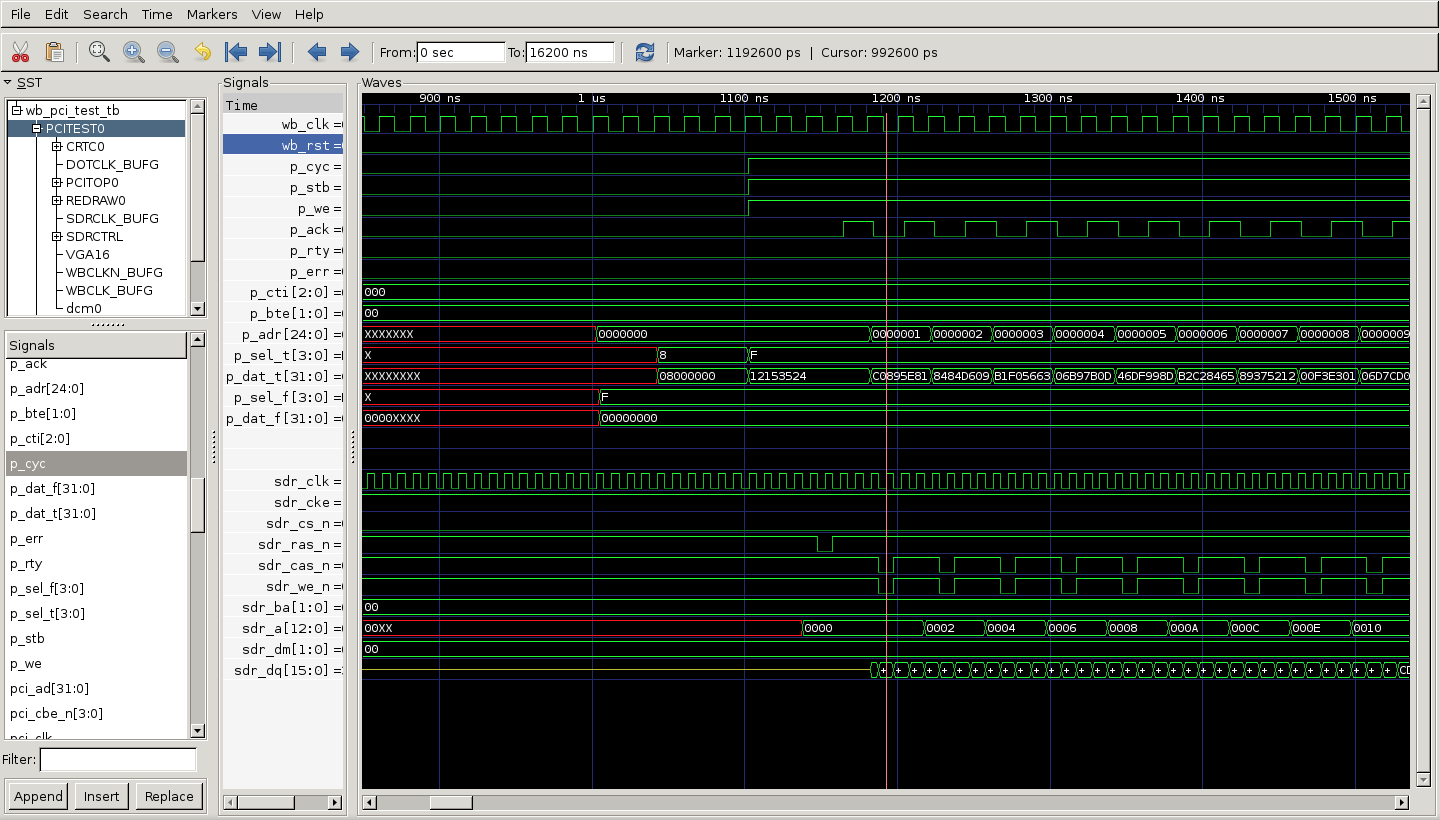
\includegraphics[width=\linewidth]{images/pci_to_sdram_xfer.png}
\caption[A simulation of a PCI to SDRAM data transfer]{A simulation of a PCI to
SDRAM data transfer.}
\label{MEM_GtkWave_SDRAM}
\end{figure}

Figure~\ref{MEM_GtkWave_SDRAM} is a GtkWave\footnote{GtkWave is free software and
is available from http://www.geda.seul.org/tools/gtkwave/index.html} screen
capture showing the simulation waveforms of a write-to-SDRAM transaction. The
transaction is initiated by the PCI bridge, transferred over the Wishbone bus to
the SDRAM controller. The SDRAM controller then writes this data to the SDRAM
device. This Wishbone bus transaction is a non-burst transfer (as determined by
the Wishbone signals \texttt{CTI} and \texttt{BTE}).

\begin{figure}[h!]
\begin{center}
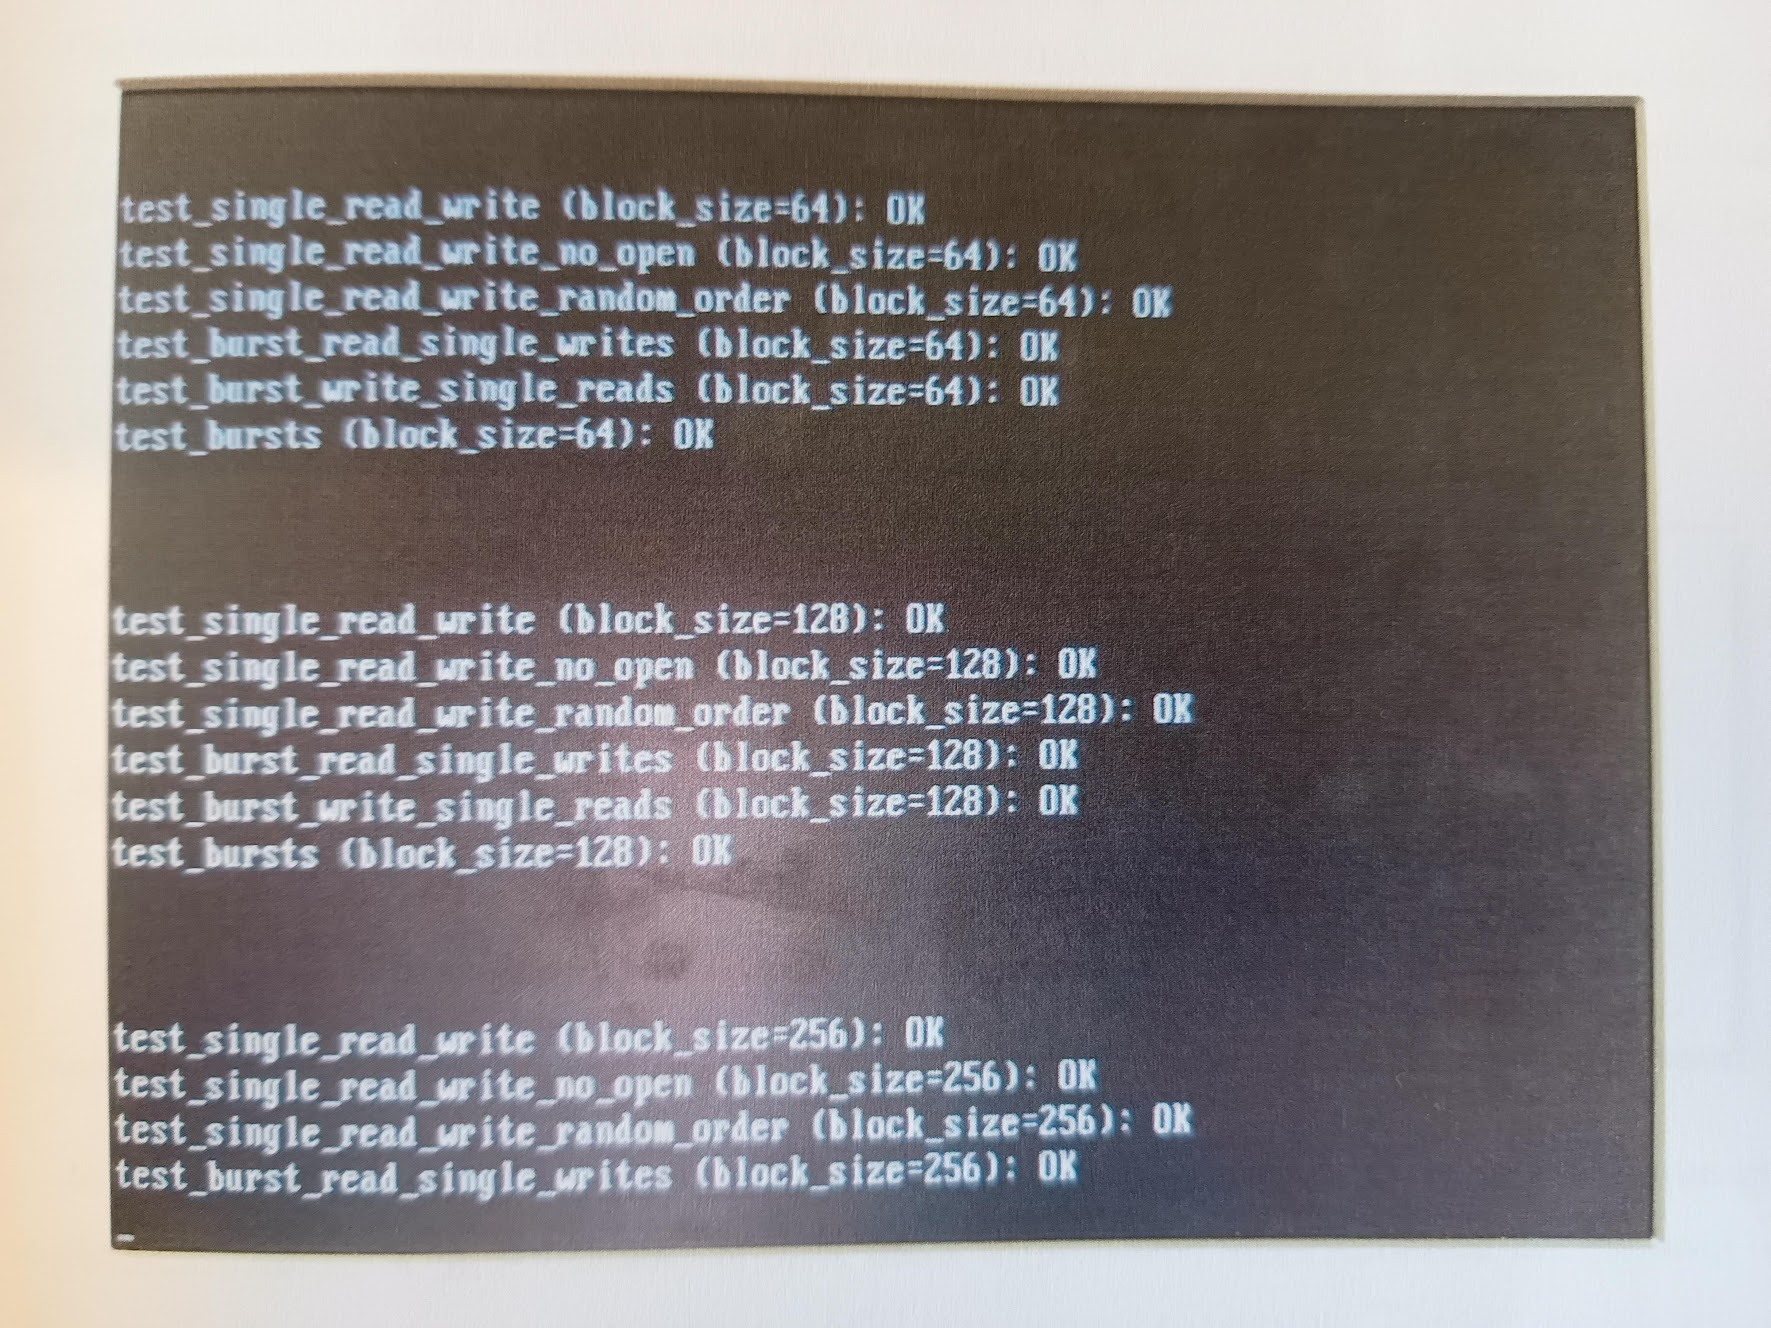
\includegraphics[width=\linewidth]{images/mem_test.jpeg}
\caption[SDRAM Memory Test Results]{OpenVGA passing memory tests
while running at 120 MHz.}
\label{MEM_Testing}
\end{center}
\end{figure}

A hardware testbench which only contained a subset of OpenVGA logic cores was
used when developing the SDRAM controller. A Linux kernel module for this
hardware testbench so that it could be accessed for testing using system API
calls. This module later became the OpenVGA kernel module.

The testing procedure consisted of writing blocks of data, of various block
sizes, and write orders, and with different transfer modes, and then reading back
and checking the data. The design passed memory tests without data corruption at
up to 120 MHz (see Figure~\ref{MEM_Testing}).


\subsubsection{Known Bugs}
\label{SDRAM_Bug}

There exists just one known bug with the SDRAM controller and this has been
narrowed down to a problem with write transactions. The system occasionally hangs
when performing large PCI burst-write transfers to OpenVGA. From the tests
performed, the following is known about this bug:

\begin{itemize}
  \item This bug is intermittent. There seems to be a small probability of it
  occurring for any PCI write transactions with a burst length of more than 256
  bytes.
  \item It occurred at all of the frequencies and memory timings tested, from
  25~MHz to 120~MHz, and with column address strobe latencies of 2, 2.5, and 3.
  \item Only occurs when the SDRAM controller logic core is used, other memory
  cores have not demonstrated this bug.
  \item It has only occurred during write operations, all reads seem unaffected.
  \item Changing the SDRAM refresh period seems to have no effect on the
  frequency of these hangs.
\end{itemize}

The system freeze does not occur when a Wishbone SRAM logic core is used instead,
indicating the problem is with the SDRAM controller, but all simulations have
failed to reproduce this bug, and hardware testing to date yields too little
information to locate the source of this bug. The current workaround is to use
many small burst transfers, rather than a few large ones.


\section{Data Cache}
\label{MEM_Cache}

\mmodule{Patrick Suggate}{wb\_simple\_cache}
{A Wishbone-compatible, 150 MHz, Spartan-3 optimised, 2 kB data cache which also
features a fast-hit lookup path.} {/rtl/cache/wb\_simple\_cache.v,
/rtl/cache/fetch\_wb.v, /rtl/cache/tag\_ram.v, /rtl/cache/cache\_bram.v}
{/sim/mem/wb\_sdram\_ctrl\_tb.v}{GPL}

A data cache for the OpenVGA processor was developed to significantly improve
memory access performance. A large quantity of data needs to processed when
updating the contents of the frame buffer, such as when performing ASCII text to
pixel conversion. The average latency of a single SDRAM memory access is high,
about 45 processor cycles per word read or written (see
Section~\ref{CACHE_Justification}), and the processor has to stall while waiting
for the memory controller.

So that the processor's memory access operations have a high throughput, low
average access latency is required. By using a data cache, average memory access
latency, and therefore performance, is improved by a factor of about eight for
the ASCII to pixel conversion algorithm (see Section~\ref{CACHE_Justification}).

The data cache has been designed to achieve a good compromise of the following
characteristics:
\begin{itemize}
  \item Logic resources used
  \item Clock frequency
  \item Design complexity
  \item Hit-time calculation
  \item Miss penalty
  \item Miss rate
\end{itemize}

For the sample workload, converting ASCII character data into pixel data, the
cache miss rate is extremely low (0.7\%), the clock rate high ($\approx$150
MHz), the average latency is only 5.1 clock cycles, and only about 80 Spartan-3
logic slices\footnote{Slice is the term Xilinx uses for its general purpose logic
resources, and within the Spartan-3 a slice contains a four-input Look-Up
Table\glossary{name={LUT}, description={Look-Up Table}} (LUT) and two DFFs}, and
a Block RAM, are used.


\subsection{Cache Justification}
\label{CACHE_Justification}
How much of an improvement in average Clock cycles required Per
Instruction\glossary{name={CPI}, description={Clocks Per Instruction}} (CPI) does
a data cache give? First, assuming OpenVGA is operating at screen resolution of
640x480, in 16-bit colour mode (2 bytes/pixel), and with a 60 Hz redraw, the data
rate ($r_\mathrm{RD}$) is given by

\[
r_\mathrm{RD} = 640 * 480 * 2 * 60 = 36864000~\mathrm{Bs}^{-1}
\]

The SDRAM controller operates at 50 MHz, the word size is 32-bits, the maximum
burst transfer size is 512 bytes, and the memory controller's fixed access
penalty (minimum memory access time, $t_\mathrm{MA}$) at 50 MHz is another eight
cycles for reads, or four cycles for writes. The parameter $t_\mathrm{MA}$ is
subsequently assumed to be six cycles per access for simplicity, though reads are
more frequent\footnote{Using six as the average penalty results in worse
statistics for the cache, so this is not an attempt to make the cache results
appear more impressive. Also, the DMA controller can be used for data writes with
ASCII text to pixel algorithm since it is well-behaved. This reduces memory bus
congestion.}.

The total redraw transaction rate ($r_\mathrm{RT}$) is given by

\[
r_\mathrm{RT} = \frac{r_\mathrm{RD}}{512} = \frac{36864000}{512} =
72000~\mathrm{Hz}.
\]

If a transaction requires $t_\mathrm{RD}$ cycles to complete, the sum of the
fixed and per-word transfer penalties, the total Wishbone bus cycles for 60
redraws, ($T_\mathrm{WB}$) is given by

\begin{eqnarray*}
T_\mathrm{WB} & = & r_\mathrm{RT} * t_\mathrm{RD} \\
  & = & 72000 * (128 + 8) = 9792000 \\
\end{eqnarray*}

Wishbone bus congestion ($c_\mathrm{WB}$), for the Wishbone bus frequency
($f_\mathrm{WB}$) of 50 MHz, is given by

\begin{eqnarray*}
c_\mathrm{WB} & = & \frac{T_\mathrm{WB}}{f_\mathrm{WB}} \\
 & = & \frac{9792000}{5\times10^7} \\
 & \approx & 20\%
\end{eqnarray*}

This result, $c_\mathrm{WB}$, is approximate because it does not have
prefetch-overshoot and refresh cycles factored in. Average memory access latency
is affected by ($c_\mathrm{WB}$). There is a probability of 0.2 that a memory
access will have to wait for a redraw prefetch transaction to complete. The
average wait is $\frac{1}{2}t_\mathrm{RD}$ cycles.

Average memory access latency ($l_\mathrm{WB}$) in Wishbone bus cycles is given
by

\begin{eqnarray*}
l_\mathrm{WB}	& = & \frac{1}{2}t_\mathrm{RD}\times 0.2 + t_\mathrm{MA} \times
0.8 \\
& = & 68 \times 0.2 + 6 \times 0.8 \\
& = & 18.4
\end{eqnarray*}

Additional parameters affecting the average memory access latency for the
processor ($l_\mathrm{CPU}$) are
\begin{itemize}
  \item $m_\mathrm{CPU}$: RISC16 has a CPU multiplier of two. This doubles
  the average memory latency seen by RISC16.
  \item $i_\mathrm{mem}$: RISC16 has a memory instruction latency cost of four
  additional cycles, due to the interlocking and flushing mechanism used.
  \item $t_\mathrm{sync}$: An additional synchronisation cost of four
  processor clock cycles because the processor and memory operate at different
  frequencies.
\end{itemize}
Giving $l_\mathrm{CPU}$ (in processor cycles)

\begin{eqnarray*}
l_\mathrm{CPU}	& = & l_\mathrm{WB} \times m_\mathrm{CPU} + i_\mathrm{mem} +
t_\mathrm{sync} \\
				& = & 18.4 \times 2 + 4 + 4 \\
				& \approx & 45
\end{eqnarray*}

Profiling the text-mode code shows that about 900,00 memory accesses (see
Figure~\ref{Mem_No_Cache}) which shows the total accesses for 50 such
conversions) are required for the conversion of a screen full of ASCII text data
to pixel data, (640x400 resolution, 16-bit colour).

If the desired display update rate, for the ASCII to pixel transformation, is 20
Hz, for smooth scrolling, and the cost for each of the memory accesses required
is 45 CPU cycles, then 720 million CPU clock cycles will be required per second.
The RISC16 processor will not be fast enough, it only operates at 100 MHz. If a
fast cache is used, which reduces average memory access time to about 5.1 cycles,
then the 100 MHz processor will be about fast enough.

% Additionally, since the average Wishbone transfer size will be larger, due to the
% DMA controller being used for memory writes, and also the number of transfers
% fewer, a data cache will result in reduced Wishbone bus congestion too. Using a
% DMA (see Section~\ref{MEM_DMA}) for writing to the SDRAM will only be more
% efficient when the write behaviour is well behaved. A large percentage of the
% entries within a cache line are modified, but since the text mode code is very
% sequential, this can safely assumed.
% 

\subsection{Implementation Considerations}
The Spartan-3 FPGA architecture has 2 kB BRAMs, which are built-in primitives,
and are suitable for implementing small caches. Each BRAM has two independent
ports and supports several different data widths. Due to the locations of the
BRAMs within the Spartan-3, aligned in two vertical columns on either side of the
FPGA, half in each column, two or more BRAMs can be connected in parallel to give
greater capacity, data transfer rates, and widths.

To design an efficient cache, the performance effects of set associativity, write
policy, capacity, data widths, line size, and replacement policy were examined.
The processor within OpenVGA has the primary purpose of converting data into a
format suitable for displaying, and for this particular application, memory
access consists of reading blocks of data, applying a transformation, and writing
the output to the framebuffer.

This sequential, block-reading/writing behaviour was speculated to heavily
benefit from a cache, since there is a high probability the next datum to be
read/written will be from one of the blocks currently cached. Furthermore, such
sequential behaviour should mean that small cache sizes will not reduce
performance much.

Factors responsible for performance when designing caches are:
\begin{itemize}
	\item Reducing the miss penalty.
	\item Reducing the miss rate.
	\item Reducing hit calculation time.
\end{itemize}
A cache that excels at all of these may well be too large to fit within the
200k-gate Spartan-3 FPGA used. To design a cache that gives good performance
without being too large, some objective measure of cache performance is needed.

Since designing and implementing a fast cache can also be very time-consuming, a
parameterisable cache simulator was written in C++ (see
Appendix~\ref{CODE_Cache}). This allows cache design parameters to be chosen
before the cache is constructed. Simply modifying the simulator parameters and
(re)running a test allows a different cache design to be evaluated. By
methodically changing each of the parameters, a cache has been chosen that will
perform well for the simulated task.

If an unrealistic simulation model is used for evaluating cache performance, due
to poor understanding of the problem, then the chosen parameters may not be
suitable for final cache design. The simulation model used for evaluating cache
performance was the ASCII text to pixel conversion algorithm, this was
implemented in C++ too (see Appendix~\ref{Source_Code}. The C++
implementation of this algorithm closely matches the desired characteristics of
the assembly routines that need to be written for the RISC16 or TTA16 processors.


\begin{figure}[h!]
\begin{center}
% \shadowbox{%
\Ovalbox{%
	\begin{minipage}{0.9\linewidth}
		\begin{center}
		\begin{minipage}{0.8\linewidth}

\begin{verbatim}

		Memory Statistics:
		Reads:		19280100
		Writes:		25684152
		Total:			44964252

		Total CPU memory access cycles: 2113319844 (Av: 47.0/op)

\end{verbatim}
		\end{minipage}
		\end{center}
	\end{minipage}}
\caption[Text-mode simulator without a cache]{Text-mode simulator output without
using a cache.}
\label{Mem_No_Cache}
\end{center}
\end{figure}

\begin{figure}[h!]
\begin{center}
\Ovalbox{%
	\begin{minipage}{0.9\linewidth}
		\begin{center}
		\begin{minipage}{0.8\linewidth}
\begin{verbatim}

Cache Properties:
    Cache Size:           2048
    Tags per Bank:          16
    Set associativity:   2-way
    Line (Block) Size:      64
    Write Policy:         thru

Memory Statistics:
Reads:		7812096
Writes:		28882131
Total:			36694227

Cache Statistics:
Accesses:	67364279
Hits:		67120151 (99.6%)
Fast Hits:	61714821 (91.9%)
Misses:		244128	(evicts = 0)
Miss rate(per 1000):	3.6

Total CPU memory access cycles:	358827429 (Av: 5.3/op)

\end{verbatim}
		\end{minipage}
		\end{center}
	\end{minipage}}
\caption[Text-mode simulator with a cache]{Text-mode simulator output when using
a cache.}
\label{Mem_With_Cache}
\end{center}
\end{figure}


\subsection{Set Associativity}
\label{CACHE_Associativity}
The set-associativity cache parameter represents how many cache look-up indices
are hashed from an incoming address. These indices are used to retrieve
cache-line tags for comparison with the incoming address. A cache with higher
set-associativity has a higher hit-rate, but also has larger and more complicated
cache sense logic.

A cache look-up consists of:
\begin{itemize}
  \item Hashing the incoming address to generate an index into the tag memory.
  \item Retrieving the tag from the tag memory.
  \item Comparing the tag-field of the incoming address to the retrieved tag.
  \item Signalling a hit and retrieving the data from cache upon a match, or
  else signalling that a miss has occurred.
\end{itemize}

With a direct-mapped cache, the incoming address can be hashed to only one
cache memory location, so there is only one tag to check. If the incoming
address is hashed to produce two different indices into the cache memory,
which data (if any) chosen depends on if either retrieved tag matches. Such a
cache design is said to be a two-way set associative cache. With two tag
banks, these two tag comparisons typically happen in parallel\cite{Comp_Arch}.

A fully associative cache requires that every tag be checked for a match. This
requires a lot of parallel comparison logic and tag memory bandwidth, and is
quite rare\cite{Comp_Arch}. Caches can be designed to be direct-mapped, or fully
associative, or anywhere in between these two extremes.

Fully associative caches typically have the highest hit
rates\cite{parhami2005cam}, if all other parameters held constant, since data can
be stored anywhere within the cache and the cache is free to choose any line to
evict. Direct-mapped caches have the lowest hit performance, but also the lowest
implementation cost (complexity, logic, and latency)\cite{Comp_Arch,
parhami2005cam}.

A two-way set associative cache was chosen since this is typically a good
trade-off for a small caches. It requires only one extra $n$-bit comparator and a
few extra logic gates, compared to a direct-mapped cache, and results in lower
miss-rates\cite{parhami2005cam}. A four-way set-associative cache would require
two more comparators than a two-way cache, and extra tag memories, and have a
higher latency on a Spartan-3 FPGA\footnote{The extra tag memories would be
needed because the Spartan-3 FPGA family has distributed RAMs with 16 entries. To
store the 32 tag entries, as determined later in this section, would require a
exactly two banks of distributed RAM for either a direct-mapped or two-way set
associative cache, but moving to a four-way set associative cache would require
two more banks of distributed memory, if simply to provide the required number of
memory read ports.}.



\subsection{Cache Size}
The results from simulating the text-mode redraw algorithm (see
Table~\ref{Mem_Cache_Size}) show that performance is extremely good with even
relatively small cache sizes because the total size of the read-data is quite
small, 2 kB of font data, 4 kB of text-mode frame buffer data, and some stack
reads.

\begin{table}[h!]
\begin{center}
% \begin{tabular}{| c | c | c | c | c |}
\begin{tabular}{ r  r  r  r  r }
% \hline
Cache & Lines   & Misses  & Miss Rate  & Average \\
Size  & (total) & (total) & (per 1000) & Latency \\
\hline
1 kB  &  16 & 485065 & 25.2 & 5.9 \\
2 kB  &  32 &  14255 &  0.7 & 5.1 \\
4 kB  &  64 &   2633 &  0.1 & 5.1 \\
8 kB  & 128 &     97 &  0.0 & 5.1 \\
16 kB & 256 &     97 &  0.0 & 5.1 \\
% \hline
\end{tabular}
\caption[Cache size vs. performance]{Performance effects of different cache
sizes, with a two-way set associative, 64 byte line size, write-through cache.}
\label{Mem_Cache_Size}
\end{center}
\end{table}

Based off these results, 2 kB, the size of a Spartan-3 BRAM, appears to be a good
choice. There is little advantage, FPGA resource usage-wise, for going smaller.
With sizes greater than 2 kB there is no significant average latency improvement,
and the extra complexity and resource usage of larger caches is of minimal
benefit in this application.


\subsection{Cache Line Size}
Shorter lines for a given size of cache require more entries within the cache
lookup table. Longer cache-lines mean that more data has to be fetched from main
memory, but the hit rate for subsequent sequential accesses will be higher.

\begin{table}[h!]
\begin{center}
\begin{tabular}{r r r r}
Line Size & Lines   & Miss Rate  & Average \\
 (bytes)  & (total) & (per 1000) & Latency \\
\hline
8   & 256 & 1.9  & 5.2 \\
16  & 128 & 1.2  & 5.2 \\
32  & 64  & 0.8  & 5.1 \\
64  & 32  & 0.7  & 5.1 \\
128 & 16  & 1.1  & 5.2 \\
256 & 8   & 3.4  & 5.4 \\
\end{tabular}
\caption[Cache line-size vs. performance]{Performance effects of different
cache line sizes, with a two-way set associative, 2 kB, write-through cache.}
\label{MEM_Line_Size}
\end{center}
\end{table}

The 2 kB data cache demonstrates excellent performance with all tested line-sizes
(see Table~\ref{MEM_Line_Size}), but the number of tags to store doubles as the
line-size halves, for a given cache size. Since a single Spartan-3 distributed
RAM has 16 entries, and there are two tag banks within a two-way set associative
cache, this means that a line size of 64~bytes is the most efficient hardware
implementation, as well as having a slight performance edge. A line size of
64~bytes was chosen for the final cache.


\subsection{Replacement Policy}
To determine which cache line to evict on a data miss, three cache data
replacement policies were evaluated:
\begin{itemize}
 \item Least Recently Used (LRU)
 \item First In, First Out (FIFO, also called round-robin)
 \item Random
\end{itemize}

Results from the cache simulator (see Figure~\ref{Mem_OpenVGA_Evict_Policy})
agreed with published results for simulations done with an Alpha 21264
processor\cite{Comp_Arch} (see Table~\ref{Mem_Alpha_Evict_Policy}).

\begin{table}[h!]
\begin{center}
% \begin{tabular}{| c | c | c | c |}
\begin{tabular}{r r r r}
% \hline
Size & LRU & Random & FIFO \\
\hline
16 kB & 114.1 & 117.3 & 115.5 \\
64 kB & 103.4 & 104.3 & 103.9 \\
256 kB & 92.2 & 92.1 & 92.5 \\
% \hline
\end{tabular}
\caption[DEC Alpha 21264 cache eviction policy vs. performance]{Different
cache eviction policies, with a two-way set associative cache, and their effect
upon cache miss rate, per 1000 instructions, with a DEC Alpha 21264 processor
running the SPEC2000 benchmarks\cite{Comp_Arch}.}
\label{Mem_Alpha_Evict_Policy}
\end{center}
\end{table}

\begin{table}[h!]
\begin{center}
\begin{tabular}{l r r}
Replacement Policy & Miss Rate & Average \\
 & (per 1000) & Latency \\
\hline
Least Recently Used & 0.8 & 5.1 \\
Random & 0.7 & 5.1 \\
First-In, First-Out & 0.8 & 5.1 \\
\end{tabular}
\caption[Cache eviction policy vs. performance]{Different cache replacement
policies and the effect on miss-rates and average latencies when simulated
using the text-mode redraw algorithm and a 2 kB, two-way set associative, 64
byte line size, write-through, data cache.}
\label{Mem_OpenVGA_Evict_Policy}
\end{center}
\end{table}

Random replacement was therefore chosen since it is the easiest to implement. The
random replacement selector is a single bit of a seven bit LFSR, as LFSRs have
been shown to generate good approximations of random
sequences\cite{dufaza1991lbd}.


\subsection{Write Policy}
The two approaches with writes to the cache are to attempt to write it straight
away (the write through policy), or store incoming data in the cache so that it
can be written to the memory in bursts. The second approach, the write back
policy, was less efficient in this case (see Table~\ref{Write_Policy}), and is
more complex to implement, so the data cache uses write though instead.

Since the majority of data written with the cache simulator, and simulating the
text to pixel conversion algorithm, uses writes to the DMA controller, not direct
memory writes, the performance of each approach will not have a significant
effect in this case anyway.

\begin{table}[h]
\begin{center}
% \begin{tabular}{| c || c | c || c | c |}
\begin{tabular}{r | r r | r r }
% \hline
Line Size & Write Back & & Write Through & \\
(bytes) & Misses/1000 & Cycles/Op & Misses/1000 & Cycles/Op \\
\hline
8   &  75.0 &  8.7 & 1.9 & 5.2 \\
16  &  37.9 &  7.1 & 1.2 & 5.2 \\
32  &  19.3 &  6.3 & 0.8 & 5.1 \\
64  &  10.9 &  6.0 & 0.7 & 5.1 \\
128 &   9.5 &  6.2 & 1.1 & 5.2 \\
256 &  20.2 &  8.6 & 3.4 & 5.4 \\
% \hline
\end{tabular}
\caption[Cache Write Policies vs. Performance]{Different cache write policies
and line-sizes, with a 2 kB, two-way set associative cache, and their effect
upon average memory latency, and cache miss rate per 1000 instructions.}
\label{Write_Policy}
\end{center}
\end{table}


\subsection{Pipeline Length}
\label{CACHE_Pipeline}
The data cache interface to the processor needs to run at the processor frequency
to minimise latency but, since hit calculation (performed by the sense logic)
requires cache tag lookup and then address comparison, there is a large
combinatorial delay, so this logic was pipelined.

\begin{figure}[h!]
\begin{center}
\includegraphics[width=\linewidth]{diagrams/cache_sense_logic.pdf}
\caption[Simplified Schematic of the Cache Sense Logic]{Simplified schematic
showing the cache sense logic.}
\label{CACHE_Sense}
\end{center}
\end{figure}

The previous two tags used for a cache look-up operation are stored so if the
same cache tag index is subsequently used, the look-up operation will take one
less clock cycle. These are called ``Fast Hits'' in the cache simulator output,
and this was about 90\% of all hits with the cache simulations, so the average
latency saving from this optimisation is about 0.9 cycles per memory access. The
previous-tag registers have an additional purpose as well. Since tag retrieval
takes several nanoseconds, they are used as pipeline registers so the cache can
operate at a higher clock frequency.

Upon hit, the total latency is zero cycles for a fast hit and one cycle for a
normal cache hit. The miss latency is determined by the state of the SDRAM as
well as the overhead imposed by the cache, plus the signal synchronisation, in
each direction, since the memory access crosses from the processor domain
to the Wishbone bus domain and back. Minimum total latency for a read is 15
cycles plus an additional one quarter of the line size (and the processor
design adds another five), but average latency for a miss will be a lot higher
since the video redraw logic is competing for SDRAM access too.

Figure~\ref{CACHE_Sense} is a simplification the data cache sense logic. The
Wishbone signals used to initiate a cache look-up are shown on the left
(\texttt{CYC}, \texttt{STB}, \texttt{WE}, and \texttt{ADR}). The \texttt{Miss}
signal is used to initiate a fetch from memory and is only asserted by cache-read
misses, never for cache-writes. The \texttt{Hit} signal is used to complete a
cache look-up transaction.


\subsection{Testing}
The first part of testing the cache was building a software cache simulator. This
allowed evaluating changes to the design can be made quickly and the performance
implications simulated and evaluated. A text-mode conversion algorithm was
written in as well. This was used with the cache simulator to provide a realistic
test scenario, and the CRT simulator was used to verify correctness.

To hardware-test the synthesised cache, software writing to OpenVGA using
PCI-to-Wishbone bridge logic core provided a workload for the cache. All PCI
bridge transactions had to pass through the cache to access the SDRAM, and the
same memory-test applications that were written for the SDRAM controller (see
Section~\ref{MEM_Testing}) could be used.



\section{DMA Controller}
\label{MEM_DMA}

\mmodule{Patrick Suggate}{wb\_dma}
{A DMA controller for writing data in bursts to a memory controller.}
{/rtl/lib/wb\_dma.v} {/sim/lib/wb\_dma\_tb.v}{GPL}

The DMA allows a peripheral to queue up write data so that it can be written to
the memory controller as a burst transfer, improving total system memory
throughput. The DMA consists of a FIFO, using a 2 kB BRAM, to buffer data until
it is ready to be written. If the DMA has been filled with 2 kB of data, it can
optionally be re-written multiple times to any location in memory. This is useful
for clearing the OpenVGA display memory for example. Information on how to access
and program the DMA controller is contained in Section~\ref{TTAPROG_DMA} of the
TTA16 programming guide.


\section{Serial PROM}
\label{Serial_PROM}

\mmodule{Patrick Suggate}{wb\_sprom}
{A Wishbone-compatible, serial PROM read-back module designed to work with Xilinx
serial PROMs.} {/rtl/lib/wb\_sprom.v} {/sim/lib/wb\_sprom\_tb.v}{GPL}

Since the FPGA state is stored internally, using SRAM, it needs to be reloaded
every time the device is powered on. Xilinx sell a Serial Flash PROM to
accomplish this task. After the initial FPGA state is loaded from this PROM,
the user can then access the PROM and read out additional data.

When building the binary image file for the PROM contents, extra data can be
appended to the end of the PROM image file. This requires some padding
bytes and an ID pattern preceding the appended data. This can then be read back
once the FPGA performs its own initialisation.

The serial PROM is needed to store the VGABIOS ROM image and additional
processor instructions, which is transferred to SDRAM upon start-up. The VGABIOS
ROM image is 32 kB of 16-bit, x86 code which resides at address 0x0C8000 in the
OpenVGA host computer's memory address space\cite{SVGA_Book}. The purpose of
this ROM is too implement standard routines for communicating with the VGA hardware.


\subsection{Serial PROM Read-Back Considerations}
Since this is typically done only on power-on, since sequential access without
direct control of the address counter is very slow, the PROM read logic should
be small so to minimise logic usage for hardware that is used just once.

The simplest way to read data from this serial PROM is to clock the data out
into a shift register, searching first for the ID pattern to locate the
beginning of user data, then continue clocking while transferring the user data
onto the Wishbone bus and to the SDRAM.
